% Escrow Protocol — technical report
% Style: arXiv-style technical report (ruled title block, CM serif, running header)
% Build: tectonic paper.tex   (from paper/)
\documentclass[11pt,letterpaper]{article}

\usepackage[margin=1.05in,top=1.15in]{geometry}
\usepackage{amsmath,amssymb}
\usepackage{graphicx}
\usepackage{booktabs}
\usepackage{array}
\usepackage{microtype}
\usepackage{xcolor}
\usepackage{caption}
\usepackage{enumitem}
\usepackage{fancyhdr}
\usepackage{titlesec}
\usepackage[colorlinks=true,urlcolor=escorange,citecolor=escorange,linkcolor=black]{hyperref}

\definecolor{escorange}{RGB}{204,85,0}

\captionsetup{labelfont=bf,labelsep=period,font=small}
\setlist{itemsep=1pt,topsep=3pt}

% ---- running header / footer ----
\newcommand{\shorttitle}{Escrow: Trustless Milestone Settlement for Freelance Work}
\pagestyle{fancy}
\fancyhf{}
\fancyhead[L]{\small\itshape \shorttitle}
\fancyhead[R]{\small\textsc{Technical Report}}
\fancyfoot[C]{\small\thepage}
\renewcommand{\headrulewidth}{0pt}
\setlength{\headheight}{14pt}

% ---- section title style ----
\titleformat{\section}{\Large\bfseries}{\thesection}{0.7em}{}
\titleformat{\subsection}{\large\bfseries}{\thesubsection}{0.6em}{}

% ---- abstract-like block ----
\newenvironment{paperabstract}{%
  \begin{list}{}{\setlength{\leftmargin}{0.35in}\setlength{\rightmargin}{0.35in}}%
  \item\begin{center}\textbf{Abstract}\end{center}\small
}{\end{list}}

\newcommand{\titleruleblock}{\noindent\rule{\textwidth}{1.1pt}}

\begin{document}

% =====================================================================
% Title block
% =====================================================================
\thispagestyle{empty}

\begin{center}
\vspace*{0.4in}
{\titleruleblock}\\[14pt]
{\huge\bfseries Escrow: Trustless Milestone Settlement\\[4pt] for Freelance Work}\\[12pt]
{\titleruleblock}\\[18pt]

{\large
Parithosh Varma\textsuperscript{\,\textdagger}\\[4pt]
\textsuperscript{\textdagger}\,Escrow Protocol\\[2pt]
\textsuperscript{\textdagger}\,Correspondence: \texttt{\href{https://github.com/Parithosh-Varma/escrow}{github.com/Parithosh-Varma/escrow}}\\[10pt]
{\normalsize\color{gray} Version 0.2 \; $\bullet$ \; August 26, 2026}
}
\end{center}

\vspace{0.15in}

\begin{paperabstract}
Freelance work runs on an awkward bargain: someone must move first. The client who
pays upfront risks receiving nothing; the freelancer who delivers first risks never
being paid. Existing platforms resolve this with a corporate intermediary that holds
funds, adjudicates conflict behind closed doors, and extracts rents from both sides.
\emph{Escrow} replaces the intermediary with a protocol. A client locks the full
project value before work begins; funds move only upon client approval, a
deadline-enforced permissionless release, or the verdict of a commit--reveal jury.
Three commitments run through every mechanism: (1)~\emph{evidence over assertion} ---
submissions carry proof-of-work artifacts pinned by content hashes; (2)~\emph{AI as
signal, jury as verdict} --- machine checks screen every submission but a flag opens a
dispute rather than blocking payment; (3)~\emph{skin in the game without capital
lockup} --- jurors are rewarded from platform fees when they side with majorities and
slashed when they dissent, via non-transferable reputation stakes. We describe the
protocol across two modes that share one API surface: an off-chain bookkeeping mode
for development, and a live mode mirroring a Solidity implementation on Base ---
UUPS-upgradeable escrow and dispute contracts whose payout accounting we verify with a
chaos-style invariant campaign (payout conservation and earmark-vs-rescue properties
held across 187{,}500 adversarial calls), a static-analysis pass, and an end-to-end
lifecycle run that includes executing contract ownership through a timelock.
\end{paperabstract}

\vspace{0.1in}

% =====================================================================
\section{Introduction}
% =====================================================================

A strong freelancer and a serious client still cannot safely transact without a
trusted third party. The failure modes are structural: whoever acts first donates
leverage. Platforms such as Upwork resolve the standoff by concentrating custody,
adjudication, and pricing power in one company --- at the cost of opaque dispute
resolution, net-30/60 payment lag, and fees borne by both sides.

Escrow is a protocol that removes the intermediary while preserving the guarantee
that makes platforms usable: \emph{neither party can defect unilaterally}. The client
locks the full project value into escrow before work begins. Funds move to the
freelancer only when one of three things happens: the client approves a milestone; a
review timeout expires and anyone may trigger release; or a jury of peers resolves a
dispute. Table~\ref{tab:statusquo} contrasts the design with the status quo.

\begin{table}[h]
\centering\small
\caption{Comparison with traditional freelance platforms.}
\label{tab:statusquo}
\begin{tabular}{@{}lll@{}}
\toprule
\textbf{Dimension} & \textbf{Traditional platforms} & \textbf{Escrow} \\
\midrule
Custody & Corporate account & Escrow lock, contract-backed in live mode \\
Dispute resolution & Opaque internal team & Commit--reveal jury, on-chain-auditable \\
Payment timing & Net-30/60 or platform whim & Per-milestone, deadline-enforced release \\
Quality signals & Ratings after the fact & PoW evidence + AI screening before payment \\
Fee destination & Platform keeps 100\% & 50\% of fee funds juror rewards \\
\bottomrule
\end{tabular}
\end{table}

\subsection{Contributions}

\begin{enumerate}
\item \textbf{A milestone escrow protocol} with upfront all-or-nothing funding, an
explicit state machine, and permissionless timeout release --- no unilateral exit,
no frozen funds (\S\ref{sec:lifecycle}).
\item \textbf{Evidence-gated deliverable custody}: counterparty previews are
watermarked with viewer-tagged provenance and unlock to original bytes only after
settlement (\S\ref{sec:custody}).
\item \textbf{AI-assisted screening with human verdicts}: requirement-match,
plagiarism, and AI-generation checks flag submissions; flags auto-open disputes that
a commit--reveal jury decides (\S\ref{sec:submissions}, \S\ref{sec:disputes}).
\item \textbf{Juror mechanism design} funded entirely from platform fees: majority-side
rewards, minority slashing, non-transferable stakes (\S\ref{sec:disputes}).
\item \textbf{An on-chain implementation on Base} --- UUPS-upgradeable escrow and
dispute contracts with a partial-approval challenge window, timelock governance, and
a storage layout frozen and documented for V2 (\S\ref{sec:contracts}).
\item \textbf{Verification at two layers}: property-tested off-chain accounting and a
187{,}500-call adversarial invariant campaign on-chain, plus an end-to-end lifecycle
run including governance handoff (\S\ref{sec:verification}).
\end{enumerate}

\subsection{Protocol modes}

The protocol ships in two modes behind one API surface. In \texttt{CHAIN\_MODE=off},
a backend ledger holds bookkeeping custody for development and CI. In
\texttt{CHAIN\_MODE=live}, an event indexer mirrors the Base contracts into Postgres
and custody lives in the contract. \S\ref{sec:contracts} describes the on-chain
implementation; \S\ref{sec:implementation} describes the backend both modes share.

% =====================================================================
\section{Protocol Overview}\label{sec:lifecycle}
% =====================================================================

\subsection{Roles and lifecycle}

A \emph{project} contains 1--50 ordered milestones, each independently specified,
funded, reviewed, and disputable. Four actors interact with the protocol: the
\emph{client} (funds and approves), the \emph{freelancer} (executes and submits),
\emph{jurors} (adjudicate disputes), and \emph{keepers} (permissionless automation:
timeout release, phase advancement, remainder claims). Every milestone lives inside
an explicit transition table; illegal moves are rejected by construction, both in the
backend state machine and on-chain by status guards.

\begin{figure}[h]
\centering
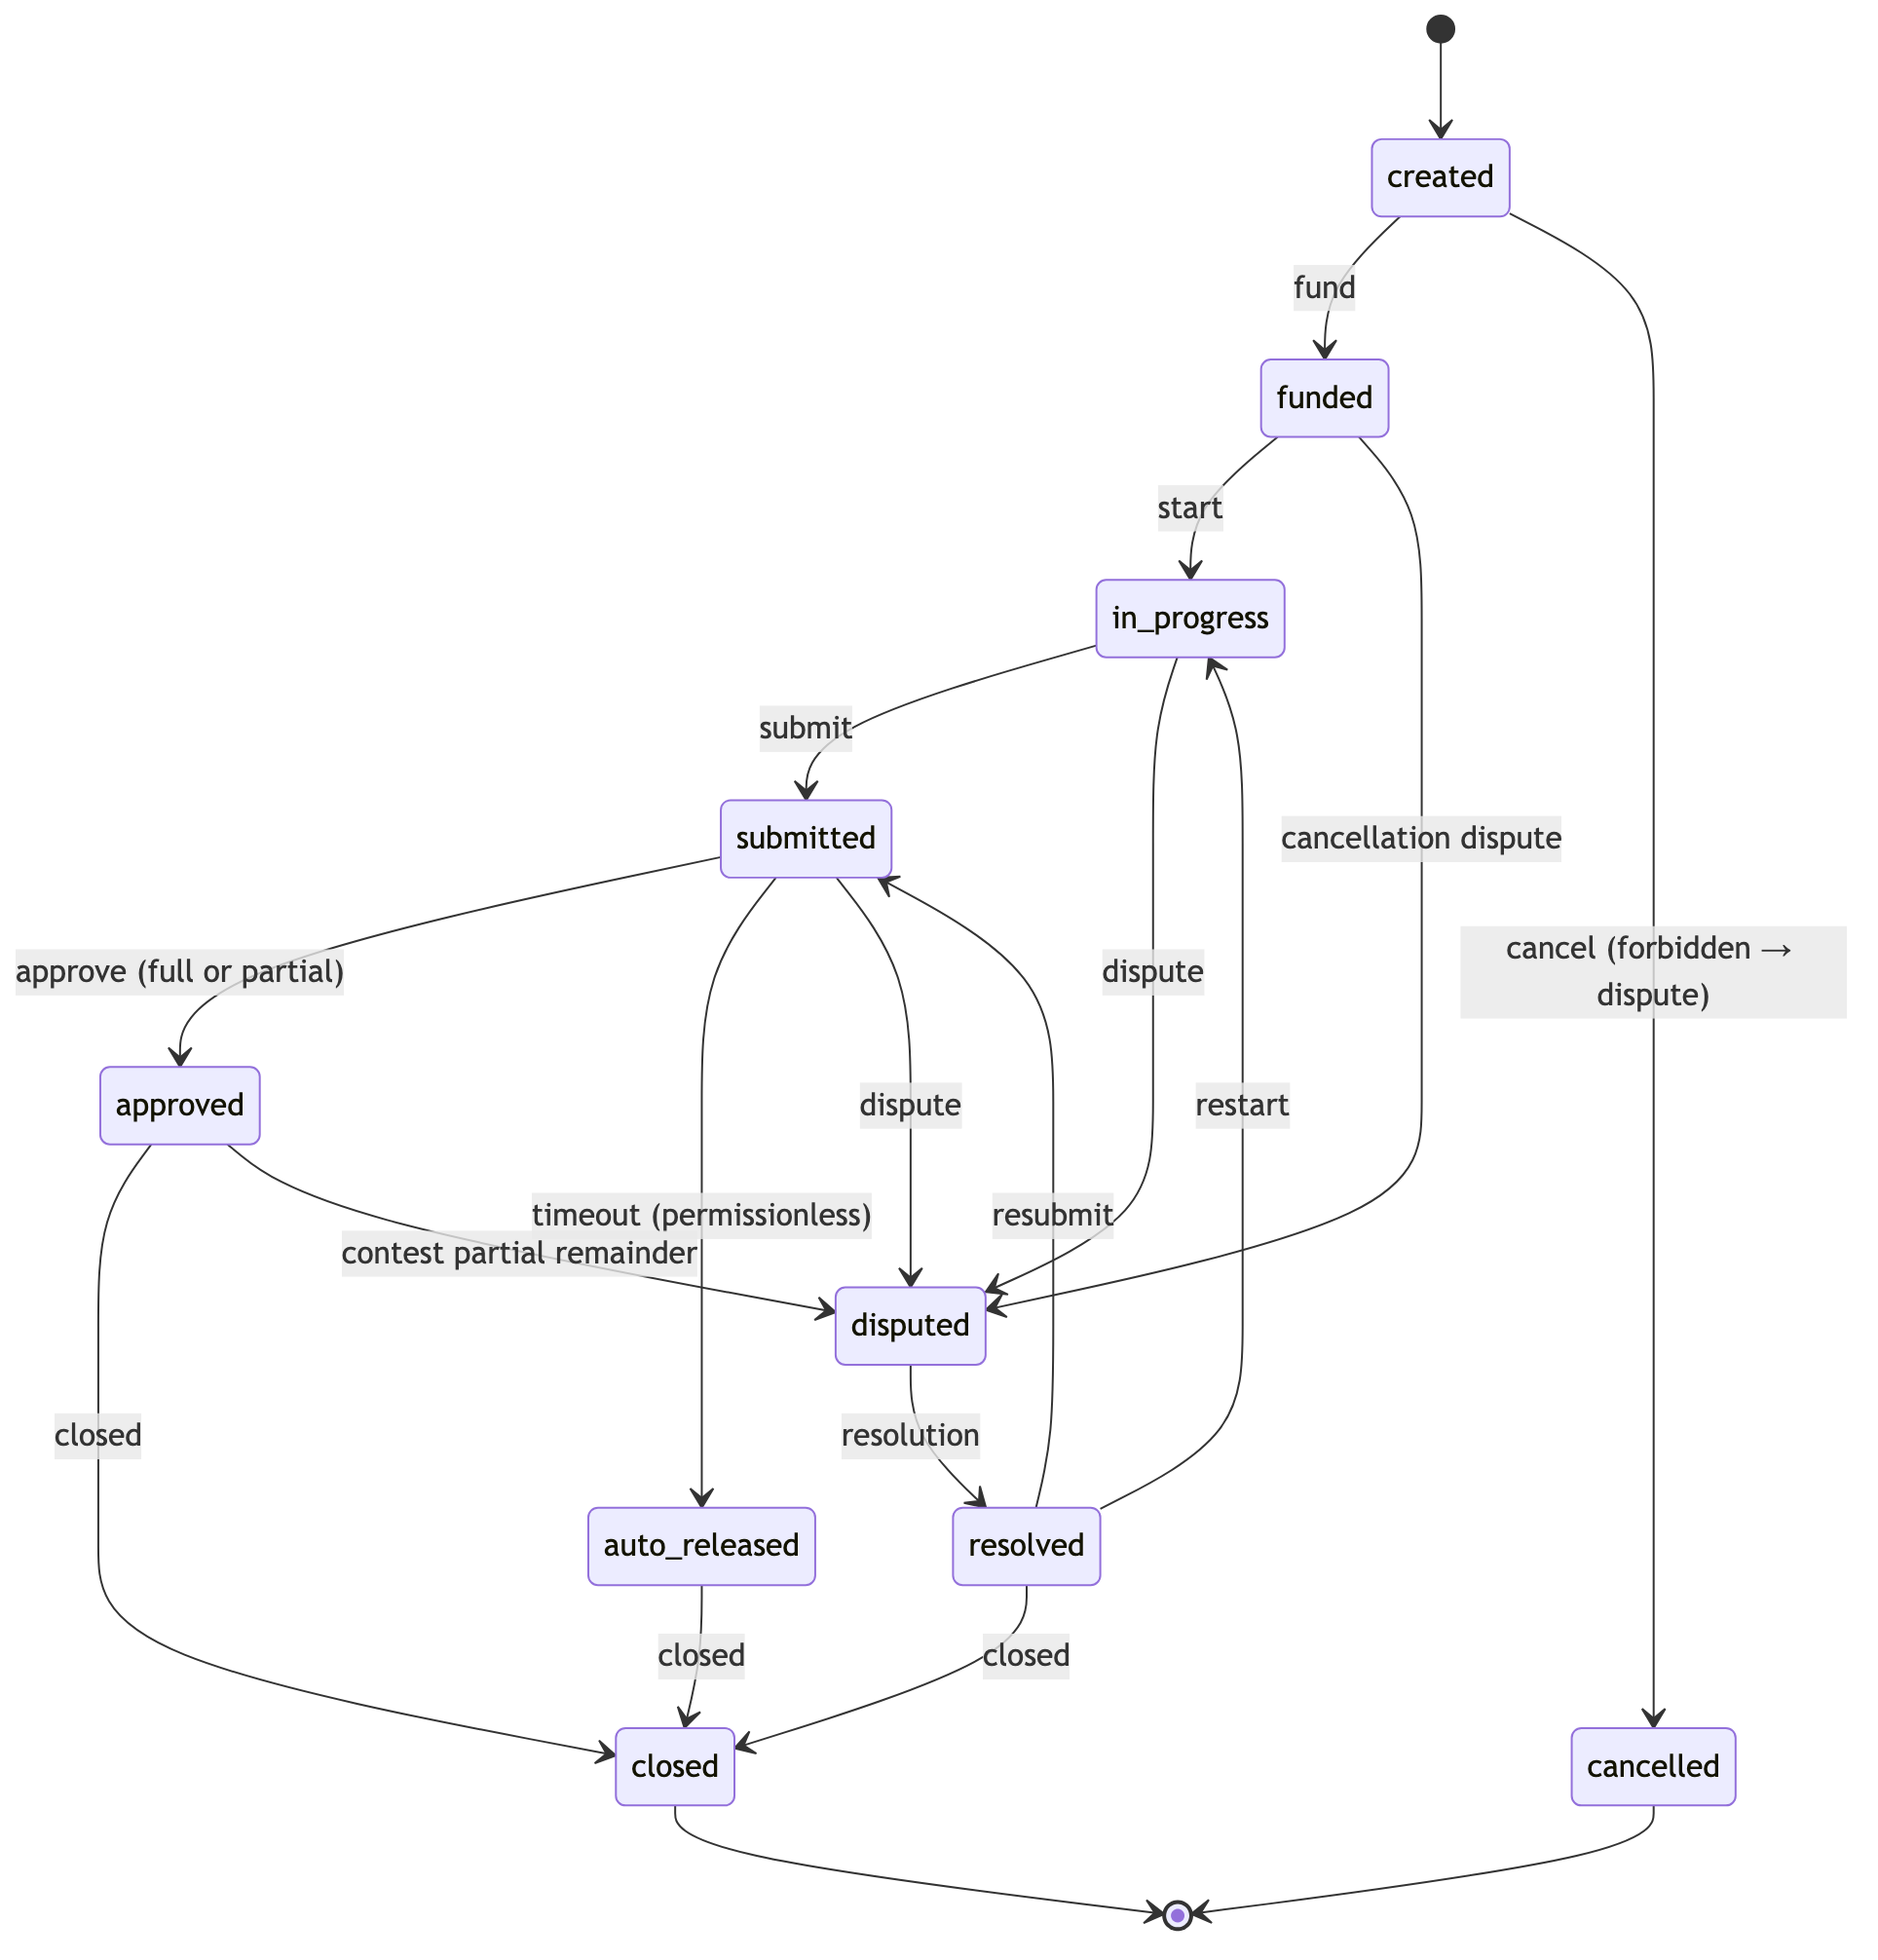
\includegraphics[width=0.62\textwidth]{diagrams/state-machine.png}
\caption{Milestone state machine. Terminal states are immutable; no unilateral
cancellation exists --- exit requires a cancellation dispute, not power.}
\label{fig:statemachine}
\end{figure}

Four properties are enforced and tested (Figure~\ref{fig:statemachine}): no state can
be skipped; terminal states are immutable; \texttt{cancel} always routes into a
\emph{cancellation dispute} rather than destroying the escrow; and partial approvals
remain contestable.

\subsection{Upfront funding}

Creation rejects self-hire, non-allowlisted tokens, and zero amounts. Funding is
all-or-nothing: an atomic conditional update flips every milestone to \emph{funded}
and writes one lock entry per milestone into the escrow account. Two concurrent
funders cannot both win; the loser finds the status already changed.

\subsection{Review window and the keeper pattern}

Submission starts a review clock (default 7 days). The client approves any share
between 1 and 10{,}000 basis points. Silence must not be a strategy: if the client
does nothing until the deadline, \emph{anyone} may trigger auto-release --- a
permissionless keeper action paying the freelancer 100\% minus the platform fee.
Because any third party can trigger it, a client cannot freeze funds by going quiet;
the network has an economic reason to keep the gears turning.

% =====================================================================
\section{Deliverable Custody: Gating and Watermarking}\label{sec:custody}
% =====================================================================

Before approval, the client must be able to \emph{evaluate} work without being able
to \emph{keep} it. This single tension produces the file system's entire design.
Files are stored content-addressed under a two-level SHA-256 key layout behind a
pluggable storage adapter --- memory for tests, disk with traversal guards for development, S3
for production. The content endpoint implements the gate shown in
Table~\ref{tab:gating}.

\begin{table}[h]
\centering\small
\caption{Access gating by viewer and milestone status.}
\label{tab:gating}
\begin{tabular}{@{}lll@{}}
\toprule
\textbf{Viewer} & \textbf{Milestone status} & \textbf{Response} \\
\midrule
Owner or admin & any & original bytes \\
Counterparty & settled (approved/released/resolved) & original bytes \\
Counterparty & anything earlier & fresh watermarked preview \\
\bottomrule
\end{tabular}
\end{table}

\begin{figure}[h]
\centering
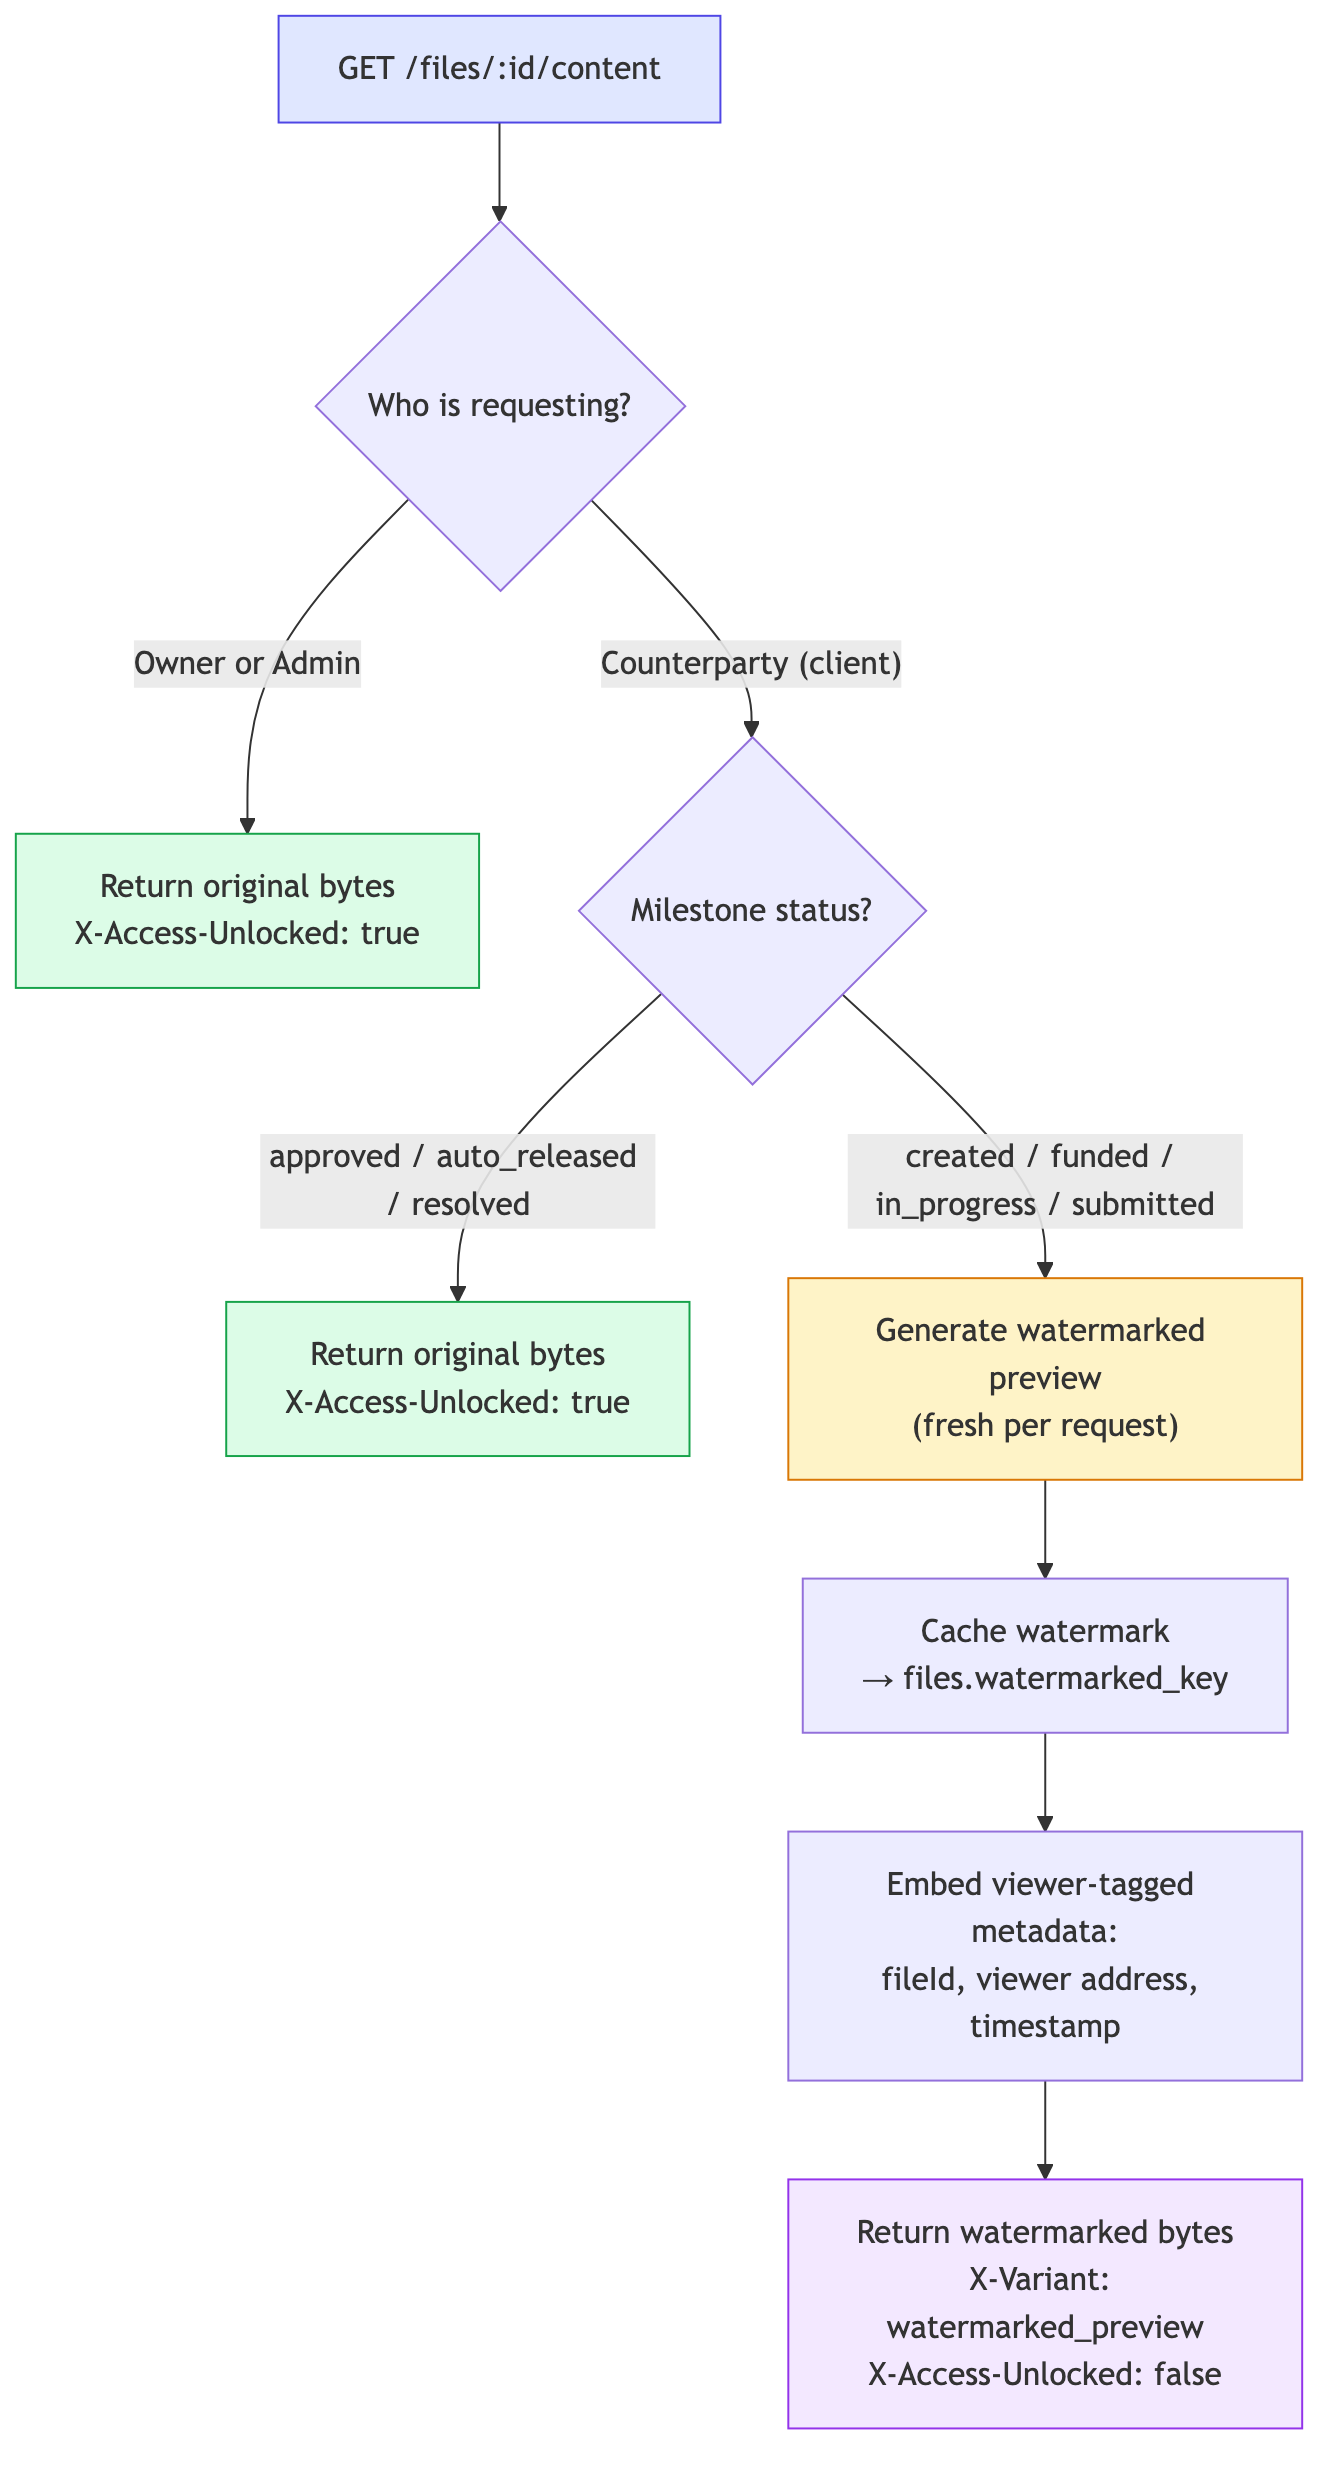
\includegraphics[width=0.6\textwidth]{diagrams/file-gating.png}
\caption{Gated custody: previews carry viewer-tagged provenance; originals unlock
only after settlement.}
\label{fig:gating}
\end{figure}

Watermarks adapt to MIME type: images receive a composited SVG overlay (bold white
text at 15\% opacity, rotated $-30^\circ$); PDFs receive a gray stamp on every page;
text-like files receive an appended HTML provenance comment; everything else a binary
trailer. Each preview embeds \emph{viewer-tagged provenance} --- file id, viewer
address, timestamp --- and is cached. If a gated deliverable leaks, the leak
identifies its viewer. Unlocked responses strip appended trailers, so delivered bytes
always differ from the canonical artifact. The gate is observable through response
headers (\texttt{X-File-Hash}, \texttt{X-Preview-Hash}, \texttt{X-Variant},
\texttt{X-Access-Unlocked}).

% =====================================================================
\section{Submissions: Proof-of-Work and AI Verification}\label{sec:submissions}
% =====================================================================

\subsection{Why submissions carry evidence}

A text message claiming completion is unfalsifiable. The submit endpoint therefore
enforces exactly one \emph{deliverable}, at least one \emph{screen recording}, and at
least one \emph{process file}. Recordings and process files show \emph{how} work was
produced --- the raw substrate jurors later inspect. The deliverable's SHA-256 pins
the submission, so what was approved is provably what was submitted.

\subsection{The three checks}

Every submission passes through three machine checks: \emph{requirement match} (does
the deliverable address the spec?), \emph{plagiarism} (is the work copied?), and
\emph{AI generation} (was it machine-generated wholesale?). Each returns a provider
tag and a confidence in $[0,1]$; a check is flagged at confidence $\geq 0.7$. Full
payloads persist for juror inspection (Figure~\ref{fig:aipipeline}).

\begin{figure}[h]
\centering
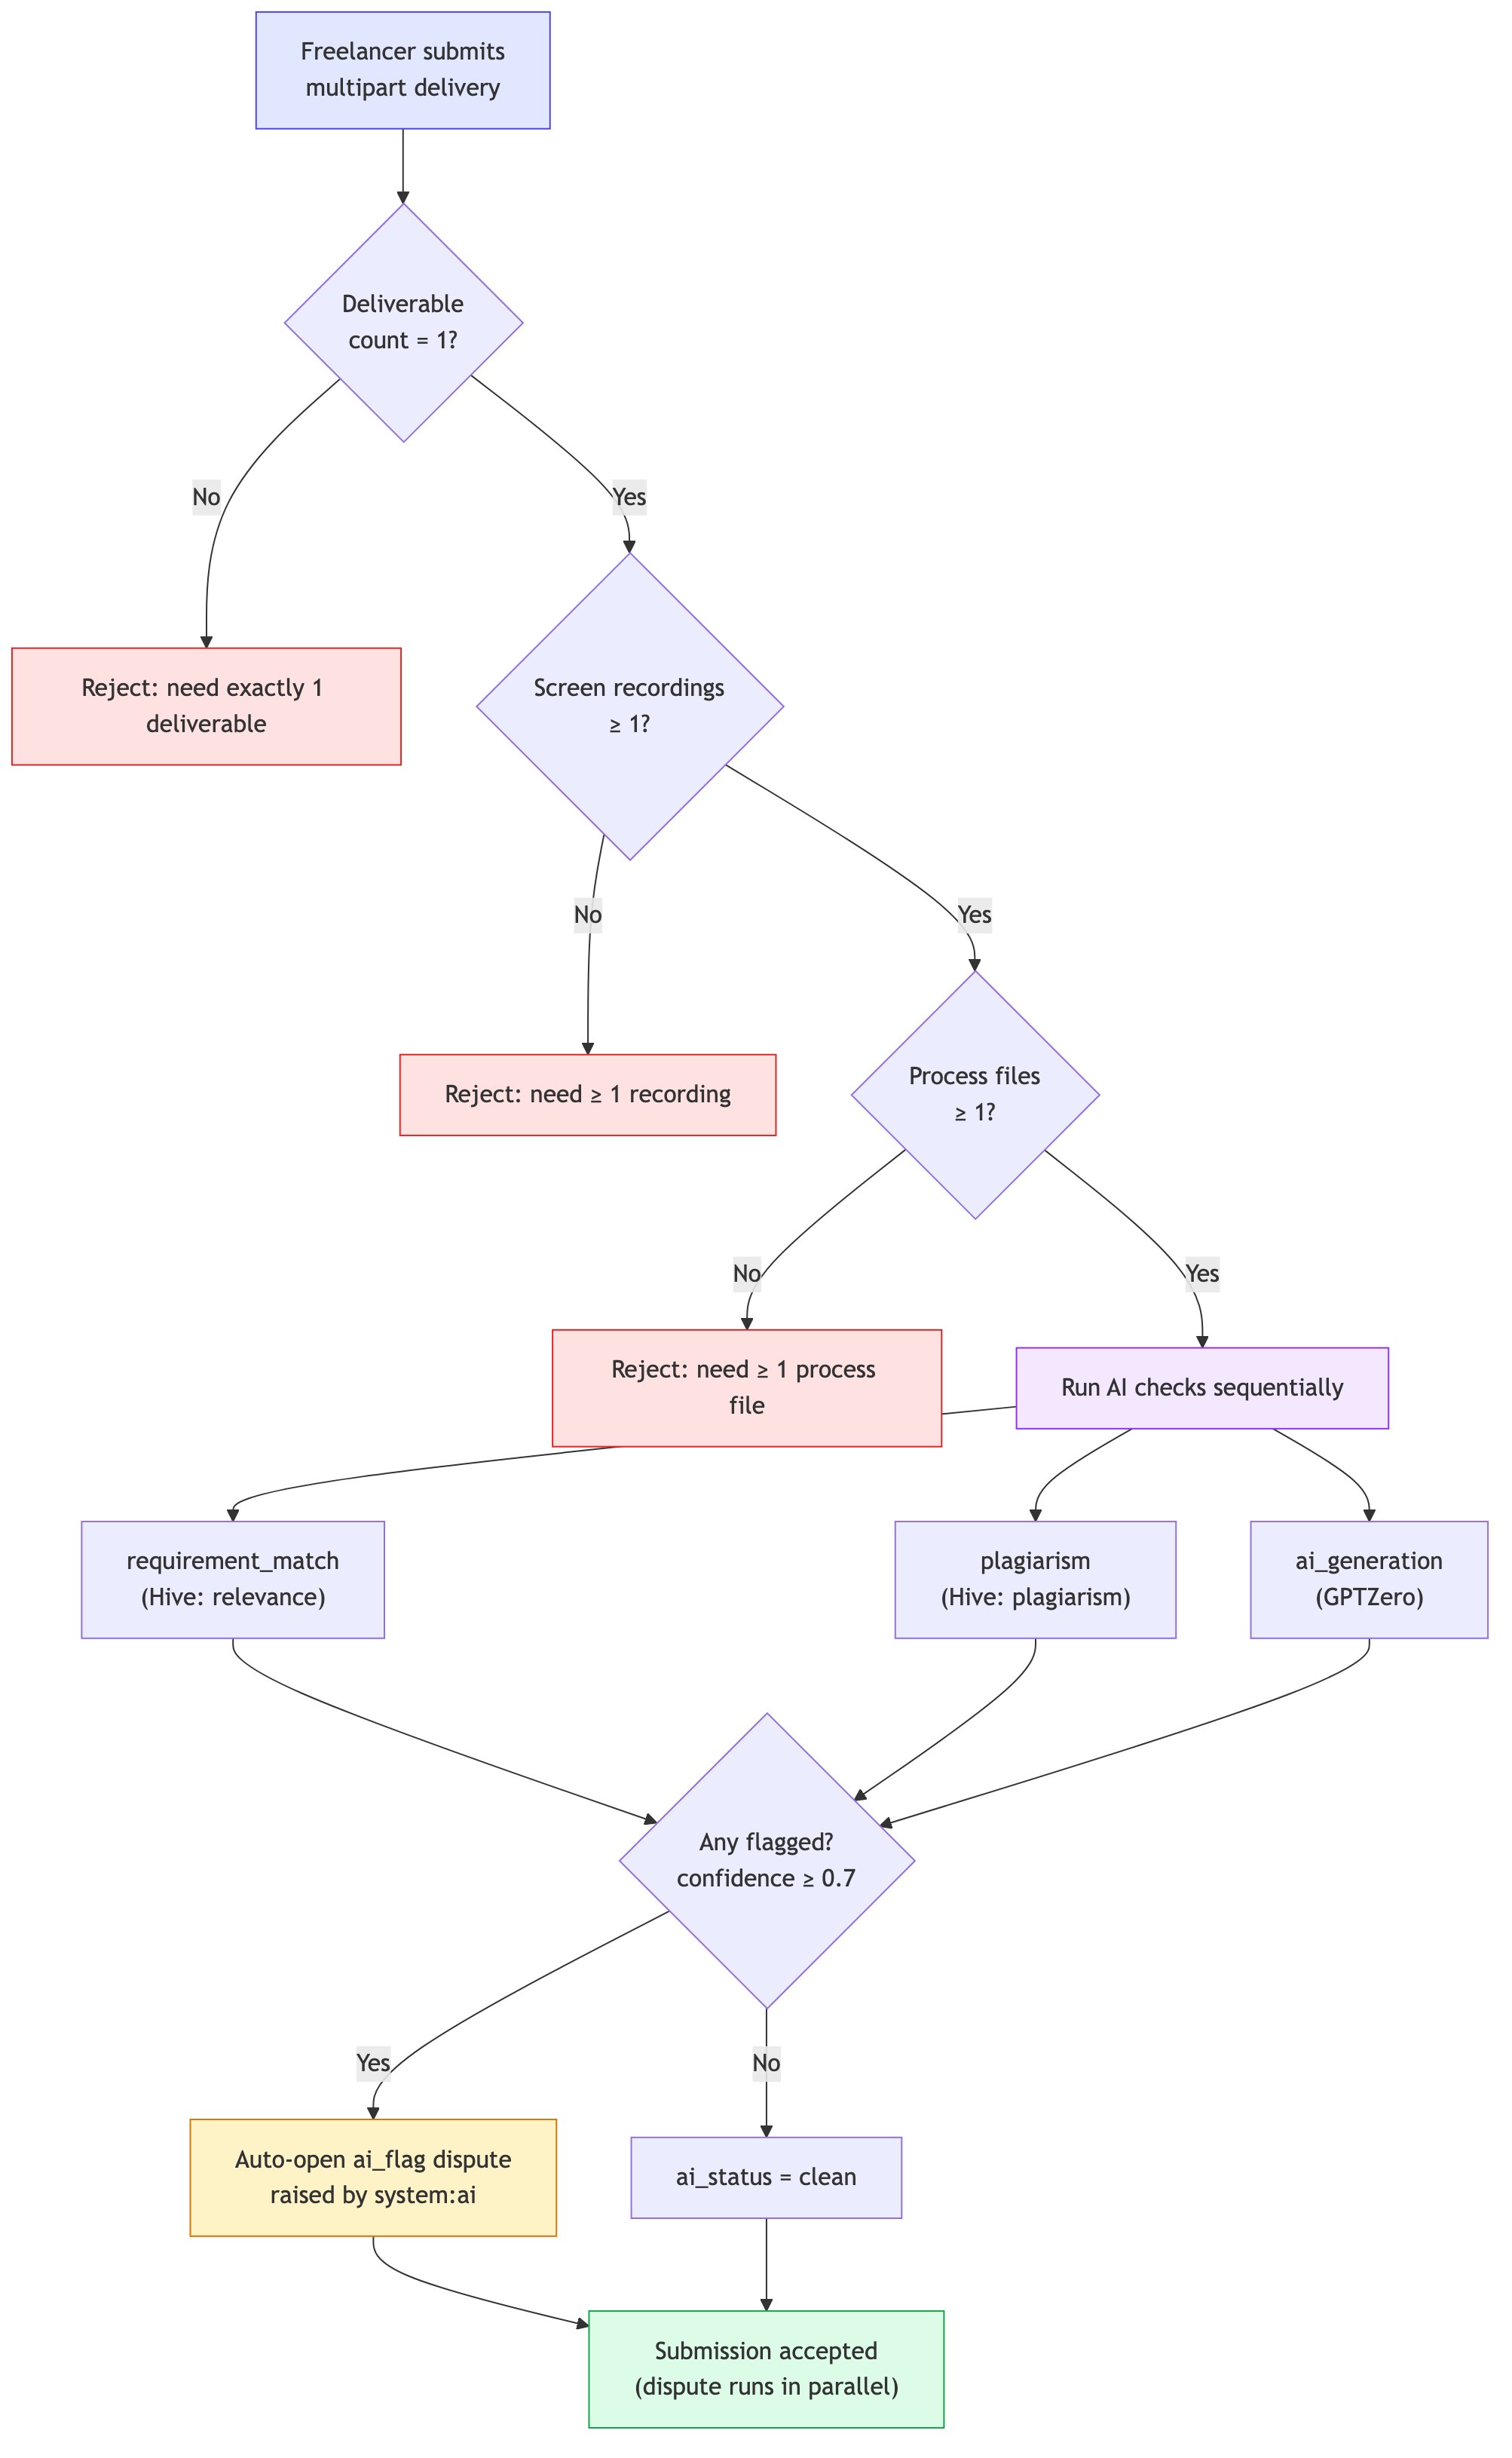
\includegraphics[width=0.66\textwidth]{diagrams/ai-pipeline.png}
\caption{AI screening pipeline. Flags open disputes; they never block payment
unilaterally.}
\label{fig:aipipeline}
\end{figure}

Checks sit behind a provider interface with a deterministic null provider for
development, an AI-text detector for generation checks, and a moderation-style API
for plagiarism. External calls carry a 30-second abort timeout and degrade to
confidence zero with the error captured --- a provider outage delays nothing.

\subsection{Flags are signals, not verdicts}

If any check flags, the system \emph{auto-opens an AI-flag dispute raised by the
system} instead of rejecting the submission. A human jury decides, informed by
machine confidence but not bound by it. Raw confidences are persisted for jurors but
masked in counterparty-facing responses --- the client sees ``flagged'', not the
exact score, preventing gaming-by-threshold-probing.

% =====================================================================
\section{Dispute Resolution}\label{sec:disputes}
% =====================================================================

\subsection{Dispute types and band-sized juries}

Only project parties may open a dispute, one open dispute per milestone. Five types
cover the failure space: \emph{quality} (work misses spec), \emph{scope} (what was
promised is contested), \emph{cancellation} (either party wants out mid-flight),
\emph{AI flag} (auto-opened by the screening pipeline), and \emph{partial amount}
(freelancer contests a partial-approval remainder, \S\ref{sec:payments}).

Jury size scales with what is at stake: disputes over at most \$500 draw 3 jurors, up
to \$5{,}000 draw 5, and anything larger draws 7. Selection draws from
admin-approved juror addresses, excludes both parties, and orders by seniority.
Phase~1 uses curated jurors; permissionless staked selection is future work
(\S\ref{sec:roadmap}).

\subsection{Juror incentives}

Jury service pays from platform revenue, never from the disputants' principal:

\begin{itemize}
\item The \textbf{reward pool} is 50\% of the platform fee on the disputed payout,
split equally among majority-side voters.
\item \textbf{Dissenters are slashed}: ten stake units (floored at zero) plus a
permanent \emph{slashed} status that blocks revealing in future disputes.
\item Stakes are \textbf{internal, non-transferable units} --- reputation, not
capital. This deliberately excludes bribery-and-buyout token economics while keeping
consequences real.
\end{itemize}

As a worked example: a 600 USDC milestone goes to dispute; five jurors commit; the
tally ends 3--2 for the freelancer. Payout: freelancer 588 USDC (98\%), platform fee
12 USDC, juror pool 6 USDC split among the three majority voters; the two dissenters
are slashed. Every number is asserted by the end-to-end suite.

\subsection{Commit--reveal voting}

Open voting fails at exactly the moment it matters: early voters anchor late ones
(bandwagoning), and once tallies leak, undecided jurors can be pressured. Escrow
therefore separates \emph{deciding} from \emph{showing} (Figure~\ref{fig:commitreveal}):

\begin{enumerate}
\item \textbf{Evidence (48\,h)} --- parties post context.
\item \textbf{Commit (24\,h)} --- each juror submits
$\mathit{commitHash} = \mathrm{keccak256}(\mathit{disputeId} \,\|\, \mathit{vote} \,\|\, \mathit{salt})$.
Votes are invisible; the dispute endpoint hides them. On-chain, commitments are bound
to the juror's address to prevent commitment copying.
\item \textbf{Reveal (24\,h)} --- jurors disclose $(\mathit{vote}, \mathit{salt})$;
the hash must match their commitment. Slashed jurors cannot reveal.
\item \textbf{Resolution} --- majority wins: freelancer majority forces a full split,
client majority forces zero, and a \emph{tie} escalates to an arbiter who may set any
graded split. Quorum, deadlines, and outcome/split consistency are enforced on-chain
even in the v1 backend-adjudicated mode.
\end{enumerate}

\begin{figure}[h]
\centering
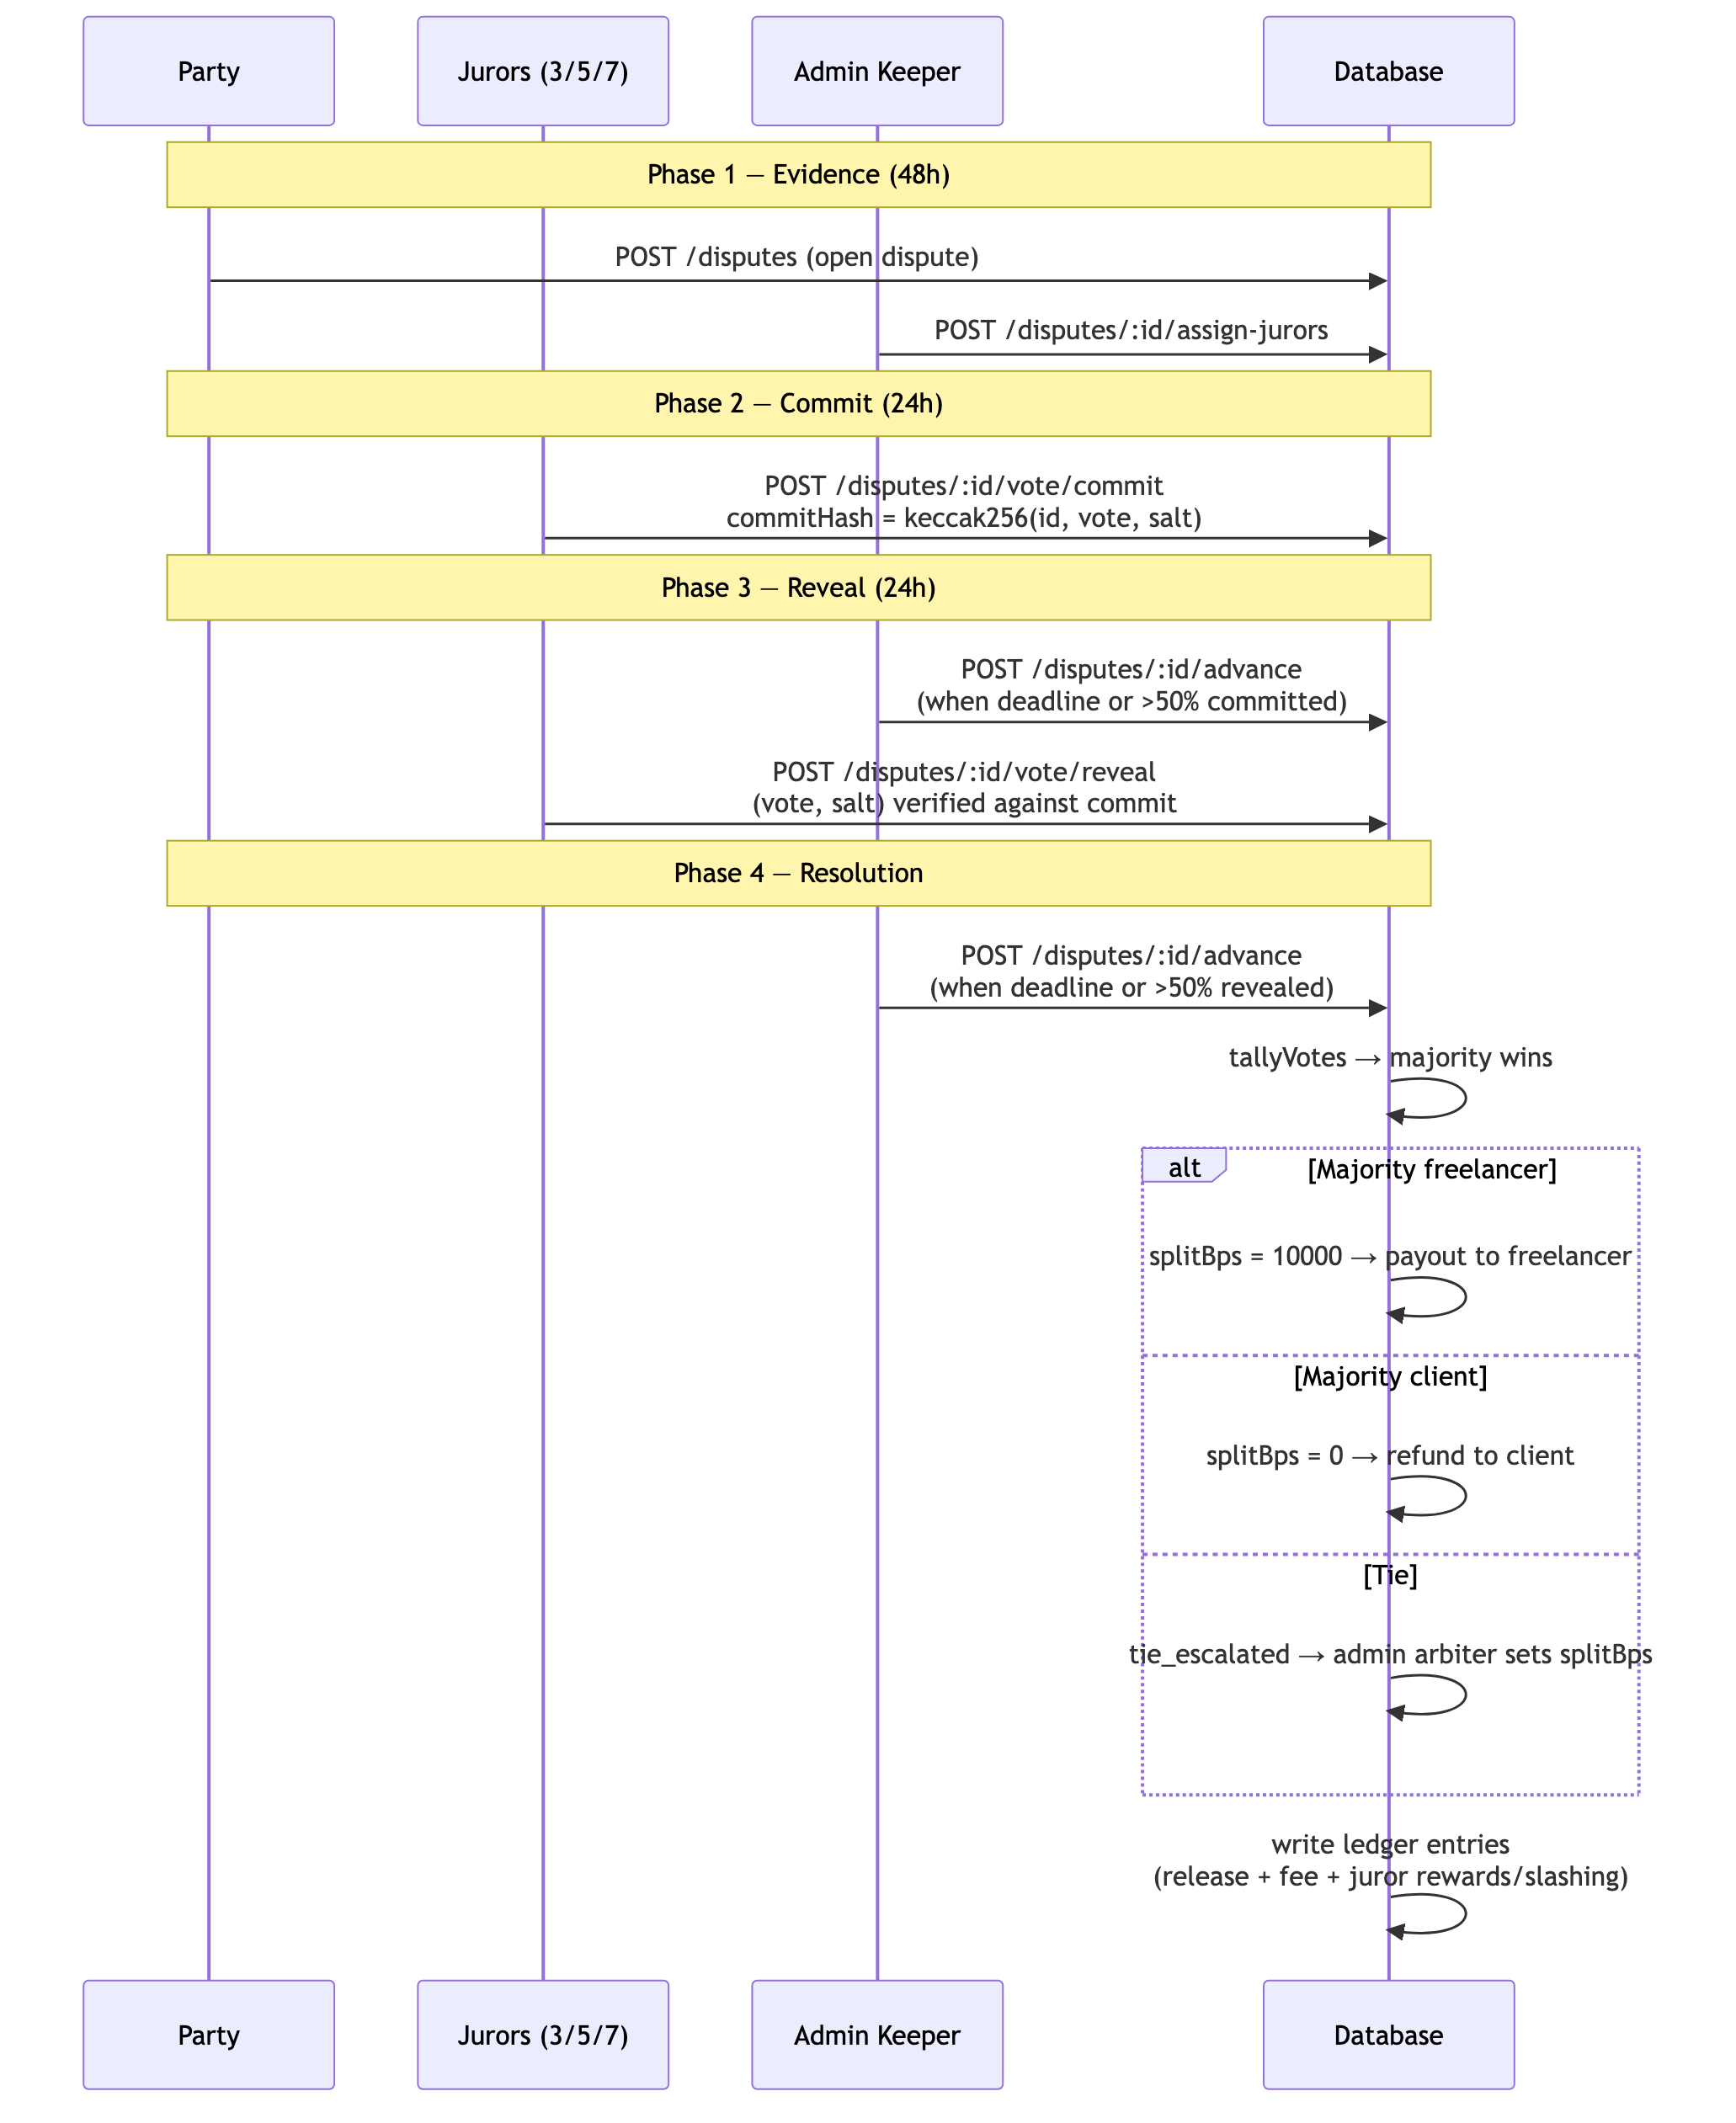
\includegraphics[width=0.62\textwidth]{diagrams/commit-reveal.png}
\caption{Commit--reveal voting. Hidden ballots prevent bandwagoning and
after-the-fact coercion.}
\label{fig:commitreveal}
\end{figure}

% =====================================================================
\section{Payments and Payout Math}\label{sec:payments}
% =====================================================================

\subsection{Money representation}

Amounts are integer base units transmitted as decimal strings and computed as
arbitrary-precision integers end to end; floating point never touches balances.
Tokens live on a curated allowlist (USDC with 6 decimals seeded for Base mainnet and
Sepolia, plus a development mock). Allowlist enforcement happens at project creation
--- no surprise token ever holds value.

\subsection{Split formula and conservation}

With milestone amount $A$, approval share $b \in [1, 10000]$ basis points, and fee
rate $f$ basis points:
%
\begin{align*}
\mathit{approvedGross} &= \lfloor A \cdot b / 10{,}000 \rfloor, &
\mathit{platformFee}   &= \lfloor \mathit{approvedGross} \cdot f / 10{,}000 \rfloor, \\
\mathit{freelancer}    &= \mathit{approvedGross} - \mathit{platformFee}, &
\mathit{clientRefund}  &= A - \mathit{approvedGross}.
\end{align*}
%
The fee floors first, so dust is never lost, and the conservation invariant
\begin{equation}
\mathit{freelancer} + \mathit{platformFee} + \mathit{clientRefund} = A
\label{eq:conservation}
\end{equation}
holds exactly for every settlement path --- approval, timeout release, and dispute
resolution alike. It is property-tested off-chain (including dust-floor cases) and
enforced continuously by the on-chain invariant campaign of \S\ref{sec:verification}
(Figure~\ref{fig:payout}).

\begin{figure}[h]
\centering
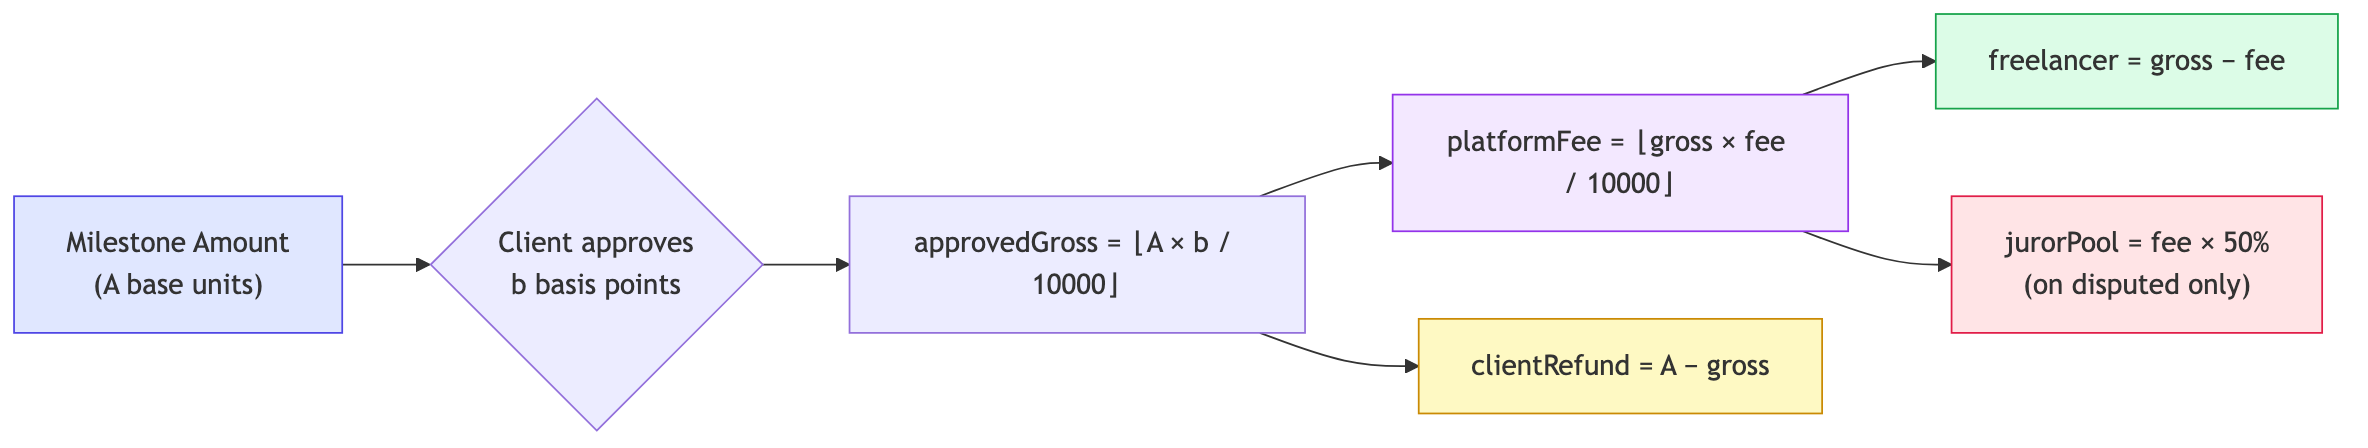
\includegraphics[width=0.5\textwidth]{diagrams/payout-split.png}
\caption{Payout split. Equation~\eqref{eq:conservation} holds on every path.}
\label{fig:payout}
\end{figure}

\subsection{The partial-approval remainder}

When a client approves fewer than 10{,}000 bps, the un-approved remainder must go
somewhere --- and where it goes decides whether the freelancer has anything real to
contest. The two modes take deliberately different policies:

\begin{itemize}
\item \textbf{Off-chain mode} refunds the remainder to the client immediately. The
freelancer retains recourse: a \emph{partial-amount} dispute whose stake equals the
refunded remainder, which a jury re-adjudicates.
\item \textbf{On-chain mode (v1 contracts)} \emph{holds the remainder in escrow}
behind a challenge window (default 7 days). Within the window the freelancer may
dispute over the held amount only --- the already-released approved portion is
untouched history. If the window expires uncontested, anyone may claim the remainder
back to the client via a permissionless keeper call.
\end{itemize}

The on-chain policy closes a real gap: a partial refund that has already left escrow
gives the freelancer nothing on-chain to dispute. Holding the remainder keeps the
stake inside the contract for the window's lifetime, and the dispute payout base is
exactly the held amount.

\subsection{Ledger design}

The off-chain ledger is append-only with fixed accounts (escrow lock, freelancer,
platform fee, client refund, juror pool) and typed entry kinds. Balances reconstruct
by summation, making any state auditable after the fact; consistency under concurrent
approvals is stress-tested. On-chain, the earmark ledger
(\texttt{totalEscrowedByToken}) plays the same role: it tracks the sum of live
allocations per token, and \S\ref{sec:verification} proves it can neither drift from
reality nor be raided by the rescue function.

% =====================================================================
\section{On-Chain Implementation}\label{sec:contracts}
% =====================================================================

The live-mode contracts are implemented in Solidity 0.8.24 with OpenZeppelin v5
upgradeable primitives and target Base, an OP-stack L2 where transaction costs make
per-milestone settlement practical.

\subsection{Architecture}

Two UUPS-upgradeable contracts behind ERC-1967 proxies share the custody logic:

\begin{itemize}
\item \textbf{EscrowCore} --- token custody, project and milestone lifecycle,
full/partial approval with the challenge window (\S\ref{sec:payments}), timeout
auto-release, dispute payout execution. Reentrancy-guarded, pausable, with a
denormalized milestone-role cache on the hot payout path.
\item \textbf{DisputeModule} --- dispute creation, band-sized juror assignment,
commit--reveal voting, phase advancement, and resolution. Quorum, deadlines, and the
outcome/split consistency rule (majority outcomes force full or zero splits; graded
splits are arbiter-only on ties) are enforced on-chain even though the v1 tally is
backend-adjudicated --- a deliberate, disclosed Phase-1 tradeoff.
\end{itemize}

Governance is a \texttt{TimelockController} (48-hour default delay) with the
multisig as sole proposer and canceller and an open executor role. Both proxies use
two-step ownership; the deployment script renounces every timelock role held by the
deployer key, so no EOA can act outside the delayed, multisig-proposed path after
handoff.

\subsection{Storage discipline for upgrades}

Both contracts reserve trailing storage gaps (43 and 44 slots) for V2 variables; the
inherited OpenZeppelin v5 state lives in ERC-7201 namespaced slots outside the
sequential layout. The full slot map --- every variable, its slot, and the rules for
appending V2 state --- is frozen in a storage-layout document that ships with the
contracts, and any upgrade PR must diff \texttt{storage-layout} output against it.
A wrong slot in an upgrade is silent fund corruption, not a revert; the document
exists so the failure mode requires ignoring a written rule, not misremembering one.

\subsection{Event surface}

{\sloppy
The indexer consumes a fixed event surface: \texttt{ProjectFunded},
\texttt{MilestoneStarted}, \texttt{MilestoneSubmitted},
\texttt{MilestoneApproved}, \texttt{AutoReleased}, \texttt{MilestoneDisputed},
\texttt{DisputeResolved}, \texttt{FundsReleased} (freelancer amount, fee, client
refund), \texttt{RemainderHeld} (with challenge deadline), and
\texttt{RemainderClaimed}. Settlement therefore spans three event types, and ids are
sequential integers --- the backend schema maps chain ids to database UUIDs at the
indexer boundary.\par}

% =====================================================================
\section{Verification}\label{sec:verification}
% =====================================================================

The protocol is verified at two layers with different failure models.

\subsection{Off-chain: property and stress testing}

Five Vitest suites (43 tests) cover the backend: end-to-end flows including a
five-juror commit--reveal dispute with exact payout assertions (588/12/6 split with
three rewarded and two slashed jurors); stress tests for auth floods, double-fund,
double-submit, and double-approve races under concurrent floods, thirty parallel
5\,MB uploads, ten parallel full lifecycles, and ledger consistency under concurrent
approvals; and unit tests for the split math including dust-floor cases and the
conservation invariant of Equation~\eqref{eq:conservation}.

\subsection{On-chain: static analysis and chaos invariants}

The contracts pass a Slither static-analysis baseline with all addressable findings
fixed (missing zero-address validation, admin state changes without events,
event-after-external-call ordering) and the remainder accepted with written
rationale (two-level bps floor division loses at most one wei per level and the
conservation identity holds by construction; timestamp dependence is inherent to
day-scale windows on an L2 with bounded sequencer drift).

The core assurance is an adversarial invariant campaign. A fuzzer drives random
interleavings of twelve handlers --- funding, progress, full and partial approvals,
timeout releases, remainder claims, dispute opening, commit--reveal resolution with
fuzzed splits, adversarial donations, surplus rescues, pausing, and clock warps ---
and after \emph{every} call asserts:

\begin{enumerate}
\item \textbf{Earmark ledger matches reality}: the per-token accounting equals the
sum of live milestone allocations (full amount while pre-settlement, held remainder
while challenge-window-held, zero once settled).
\item \textbf{Payout conservation}: the contract balance equals live allocations plus
un-rescued donations. Any double payment, leak, stuck fee, or stolen earmark makes
the balance diverge.
\item \textbf{Earmark never exceeds balance}: the rescue function can never strand
live funds.
\end{enumerate}

A meta-invariant fails the campaign if any settlement path goes unreached, so the
conservation checks cannot pass vacuously. In the heavy configuration (250 runs
$\times$ 750 calls) all four invariants hold across 187{,}500 adversarial calls.

\subsection{End-to-end lifecycle on chain}

A scripted lifecycle exercises every settlement path against deployed contracts with
per-actor keys: a project is funded; a milestone is partially approved (70\%), the
held remainder is contested through a real commit--reveal jury (two freelancer votes
to one client vote) and released in full per the majority rule; a second milestone is
fully approved; a third auto-releases after the review deadline; a fourth milestone's
remainder is claimed back after an uncontested window; a third-party donation creates
surplus and the owner rescues exactly that surplus. The run ends with the escrow
empty, the earmark ledger at zero, and every balance matching closed-form
expectations. Finally, the multisig schedules \texttt{acceptOwnership} on both
proxies through the timelock, waits out the delay, and executes --- after which the
deployer key holds no authority anywhere. The same scripts drive an anvil simulation
and a Base Sepolia deployment unchanged.

% =====================================================================
\section{Security Analysis}\label{sec:security}
% =====================================================================

\begin{table}[h]
\centering\small
\caption{Threat model and defenses.}
\label{tab:threats}
\begin{tabular}{@{}p{0.44\textwidth}p{0.5\textwidth}@{}}
\toprule
\textbf{Threat} & \textbf{Defense} \\
\midrule
Double-fund / double-submit / double-approve races & Atomic conditional updates off-chain; status guards + reentrancy guards on-chain \\
Unlisted or malicious tokens & Allowlist enforced at creation; fee-on-transfer and bad-return tokens rejected by tests \\
Path traversal on disk storage & Key sanitization + traversal guard \\
Vote manipulation, bandwagoning & Commit--reveal with address-bound commitments; votes hidden until reveal \\
Slashed jurors returning & Juror status re-read from the database on every request \\
Information leakage & Confidence masking; hidden votes; viewer-tagged watermarks \\
Client freezes funds by silence & Permissionless auto-release after the review deadline \\
Freelancer contests a lowball partial approval & Held remainder + challenge window on-chain; stake-equal dispute off-chain \\
Malicious or buggy upgrade & UUPS behind timelock; frozen storage layout with diff requirement; two-step ownership \\
Admin key compromise post-handoff & No EOA authority: all admin actions traverse the 48-hour timelock \\
\bottomrule
\end{tabular}
\end{table}

Privilege hygiene follows one rule: admin and juror claims are re-read from the
database on every authenticated request, so a revoked juror loses power mid-session
even with a valid token. Authentication is passwordless wallet sign-in --- a
single-use nonce with a ten-minute TTL and EIP-191 signature recovery --- and forged
signatures are rejected by test.

% =====================================================================
\section{Implementation}\label{sec:implementation}
% =====================================================================

\subsection{Backend}

The backend is Node 20+ with TypeScript, Fastify, Zod-validated requests
\emph{and} environment configuration, PostgreSQL via Drizzle (serverless Neon in
production, embedded PGlite for zero-config development), viem against Base, and
pluggable storage adapters. One state machine module owns every milestone
transition; one ledger module owns every balance mutation. AI providers, storage
backends, and chain configuration each degrade gracefully --- an outage in any of
them delays the lifecycle but never blocks it.

\subsection{API surface}

The HTTP surface comprises wallet authentication (challenge/verify), project creation
and funding, milestone start/submit/approve/auto-release, dispute lifecycle
(open, juror assignment, commit, reveal, advance, tie resolution), gated file custody
(upload, metadata, content), juror queues, and administration (token allowlist, juror
approval). In live mode the same routes proxy to indexed chain state; funding becomes
read-only because custody lives in the contract.

\subsection{Data model}

Core tables: users (with non-transferable juror stakes), auth nonces, token
allowlist, projects, milestones (unique per project index), submissions with
AI status and deliverable hash, files with content hashes and watermarked-variant
keys, AI check payloads, disputes with phases and splits, dispute jurors with
commitments and outcomes, append-only ledger entries, notifications, and the indexer's
cursor and idempotent event log (unique per contract, transaction hash, and log
index --- replay is safe).

% =====================================================================
\section{Limitations and Roadmap}\label{sec:roadmap}
% =====================================================================

Honest accounting of current boundaries:

\begin{enumerate}
\item \textbf{Dispute tallies are backend-adjudicated in v1.} Juror votes are recorded
on-chain as an audit trail, and quorum, deadlines, and outcome/split consistency are
enforced on-chain, but the tally itself arrives from an authorized backend call.
Acceptable for Phase 1 with curated jurors; the roadmap computes the tally on-chain
and makes resolution permissionless.
\item \textbf{Juror selection is admin-curated.} Staked, permissionless jury selection
is future work; non-participation currently emits a slash signal applied off-chain.
\item \textbf{Off-chain mode does not move tokens.} The ledger is authoritative
bookkeeping until live mode.
\item \textbf{Notifications are database rows}; email and push delivery are unwired,
and deliverable text extraction is not yet feeding the AI checks.
\item \textbf{Mainnet governance is pending} the multisig accepting ownership through
the timelock after a public testnet soak.
\end{enumerate}

The roadmap follows dependency order: live-mode cutover against the audited
contracts, on-chain tally and permissionless resolution, staked juror selection, text
extraction into richer AI checks, notification delivery.

% =====================================================================
\section{Conclusion}
% =====================================================================

Escrow demonstrates that the core promise of a freelance platform --- neither party
can defect unilaterally --- does not require a company to hold the money. Upfront
escrow removes the first-mover problem; deadline-enforced permissionless release
removes the silence strategy; evidence-carrying submissions and viewer-tagged
watermarks make quality claims falsifiable; AI screening scales review while
commit--reveal juries keep verdicts human; and fee-funded juror incentives align
adjudicators with majorities without introducing a speculative token.

The implementation is complete at both layers: a backend that runs the full protocol
off-chain today, and Base contracts whose payout accounting survived 187{,}500
adversarial calls with conservation intact, wrapped in governance that leaves no key
above the timelock. The remaining distance to production is operational --- a public
testnet soak, an external audit of the contracts, and the live-mode cutover --- not
architectural.

% =====================================================================
\begin{thebibliography}{9}\small

\bibitem{nakamoto2008} S. Nakamoto. \emph{Bitcoin: A Peer-to-Peer Electronic Cash
System}. 2008.

\bibitem{buterin2014} V. Buterin. \emph{A Next-Generation Smart Contract and
Decentralized Application Platform}. Ethereum Whitepaper, 2014.

\bibitem{eip4361} R. Gomes, P. Engel, et al. \emph{EIP-4361: Sign-In with Ethereum}.
Ethereum Improvement Proposal, 2022.

\bibitem{usdc} Circle Internet Financial. \emph{USDC Whitepaper}. 2023.

\bibitem{base} Base. \emph{Base Documentation: An OP-Stack L2 by Coinbase}. 2024.
\texttt{docs.base.org}

\bibitem{oz} OpenZeppelin. \emph{Contracts Upgradeable v5}. 2024.
\texttt{docs.openzeppelin.com/contracts-upgradeable}

\bibitem{solidity} C. Reitwiessner et al. \emph{The Solidity Language Reference,
v0.8.24}. Ethereum Foundation, 2024.

\bibitem{slither} J. Feist, G. Grieco, and A. Groce. \emph{Slither: A Static Analysis
Framework for Smart Contracts}. IEEE International Conference on Software Maintenance
and Evolution (ICSME), 2019.

\bibitem{foundry} Paradigm. \emph{Foundry: Blazing Fast, Portable and Modular Toolkit
for Ethereum Development}. 2024. \texttt{book.getfoundry.sh}

\bibitem{kleros} C. Lesaege, F. Ast, and W. George. \emph{Kleros: Short Paper v1.0.7}
--- Blockchain Dispute Resolution Layer. 2019.

\bibitem{aragoncourt} Aragon. \emph{Aragon Court: A Dispute Resolution Protocol for
Aragon Organizations}. 2020.

\bibitem{schelling} T. C. Schelling. \emph{The Strategy of Conflict}. Harvard
University Press, 1960.

\bibitem{commitreveal} Ethereum Foundation. \emph{Commit-Reveal Scheme}. Ethereum
Developer Documentation, 2024.

\bibitem{gptzero} E. Tian. \emph{GPTZero: AI Content Detection}. 2023.
\texttt{gptzero.me}

\bibitem{hive} The Hive AI. \emph{Moderation and Classification APIs}. 2024.
\texttt{thehive.ai}

\end{thebibliography}

% =====================================================================
\appendix
\section{Protocol Parameters}
% =====================================================================

\begin{table}[h]
\centering\small
\caption{Protocol parameters and defaults.}
\label{tab:params}
\begin{tabular}{@{}>{\raggedright\arraybackslash}p{0.30\textwidth}>{\raggedright\arraybackslash}p{0.24\textwidth}>{\raggedright\arraybackslash}p{0.34\textwidth}@{}}
\toprule
\textbf{Parameter} & \textbf{Default} & \textbf{Meaning} \\
\midrule
\texttt{PLATFORM\_FEE\_BPS} & 200 (cap 5000) & Platform cut per payout \\
\texttt{REVIEW\_TIMEOUT\_SECONDS} & 604800 (7\,d) & Review window before auto-release \\
\texttt{challengeWindow} & 7\,d (min 1\,h) & On-chain partial-remainder hold \\
\texttt{JUROR\_BAND\_1\_MAX} & \$500 & Jury of 3 up to this amount \\
\texttt{JUROR\_BAND\_2\_MAX} & \$5{,}000 & Jury of 5; above, jury of 7 \\
\texttt{JUROR\_POOL\_SHARE\_BPS} & 5000 & Fee share funding juror rewards \\
\texttt{SLASH\_UNITS} & 10 & Stake deducted from dissenters \\
\texttt{FLAG\_THRESHOLD} & 0.7 & AI confidence marking a check flagged \\
Evidence / commit / reveal & 48\,h / 24\,h / 24\,h & Dispute phase durations \\
Timelock delay & 48\,h (testnet: configurable) & Governance execution delay \\
\texttt{INDEXER\_POLL\_MS} & 12{,}000 & Live-mode chain poll interval \\
Nonce TTL & 10\,min & Wallet-auth challenge lifetime \\
Body limits & 100\,MB JSON / 512\,MB multipart & Generous: submissions carry recordings \\
\bottomrule
\end{tabular}
\end{table}

\end{document}
